\documentclass{article}
\usepackage[T1]{fontenc}
\usepackage{lmodern}
\usepackage{graphicx}
\usepackage{amsmath,amssymb}
\usepackage[a4paper,margin=2cm]{geometry}
\usepackage[absolute,overlay]{textpos}
\setlength{\TPHorizModule}{1mm}
\setlength{\TPVertModule}{1mm}
\usepackage[indonesian]{babel}
\usepackage{hyperref}
\setlength{\emergencystretch}{2em}
% unit: Halaman 18

\begin{document}

% === Halaman 18 (llm) ===

Akhirnya, campurkan $L$ dan $S$ sebagai berikut:

\vspace{160.38mm}

\begin{algorithmic}
\State $i \leftarrow 0$
\State $j \leftarrow 0$
\State $X \leftarrow 0$
\State $Y \leftarrow 0$
\State $n \leftarrow 3 * \max(r, c)$
\For{$k \leftarrow 1$ \textbf{to} $n$ \textbf{do}}
\State $S[i] \leftarrow (S[i] + X + Y) \lll 3$
\State $X \leftarrow S[i]$
\State $i \leftarrow (l + 1) \pmod{t}$
\State $L[j] \leftarrow (L[j] + X + Y) \lll (X + Y)$
\State $Y \leftarrow L[j]$
\State $j \leftarrow (j + 1) \pmod{c}$
\EndFor
\end{algorithmic}

% deskripsi: Potongan kode algoritma pemrosesan array L dan S dengan operasi bitwise rotation dan modulo.
% bbox normalisasi: [0.1700, 0.2600, 0.6100, 0.8000]
\begin{textblock*}{92.40mm}(35.70mm,77.22mm)
\noindent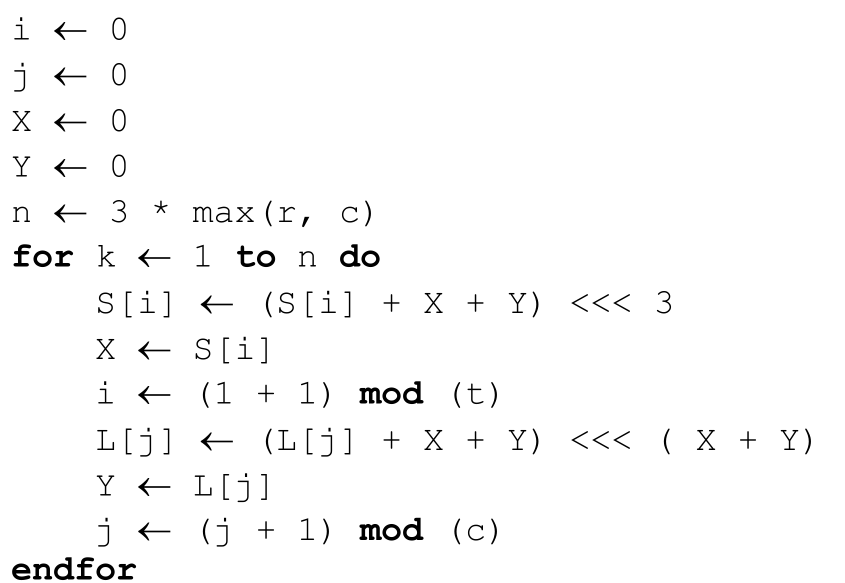
\includegraphics[width=92.40mm,height=160.38mm]{../../images/llm/page_018_img_01.png}%
\end{textblock*}

\end{document}
